%%%%%%%%%%%%%%%%%%%%%%%%%%%%%%%%%%%%%%%%%
% Jacobs Landscape Poster
% LaTeX Template
% Version 1.1 (14/06/14)
%
% Created by:
% Computational Physics and Biophysics Group, Jacobs University
% https://teamwork.jacobs-university.de:8443/confluence/display/CoPandBiG/LaTeX+Poster
% 
% Further modified by:
% Nathaniel Johnston (nathaniel@njohnston.ca)
%
% This template has been downloaded from:
% http://www.LaTeXTemplates.com
%
% License:
% CC BY-NC-SA 3.0 (http://creativecommons.org/licenses/by-nc-sa/3.0/)
%
%%%%%%%%%%%%%%%%%%%%%%%%%%%%%%%%%%%%%%%%%

%----------------------------------------------------------------------------------------
%	PACKAGES AND OTHER DOCUMENT CONFIGURATIONS
%----------------------------------------------------------------------------------------

\documentclass[final]{beamer}

\usepackage[scale=1.24]{beamerposter} % Use the beamerposter package for laying out the poster

\usetheme{confposter} % Use the confposter theme supplied with this template

\setbeamercolor{block title}{fg=ngreen,bg=white} % Colors of the block titles
\setbeamercolor{block body}{fg=black,bg=white} % Colors of the body of blocks
\setbeamercolor{block alerted title}{fg=white,bg=dblue!70} % Colors of the highlighted block titles
\setbeamercolor{block alerted body}{fg=black,bg=dblue!10} % Colors of the body of highlighted blocks
% Many more colors are available for use in beamerthemeconfposter.sty
%-----------------------------------------------------------
% Define the column widths and overall poster size
% To set effective sepwid, onecolwid and twocolwid values, first choose how many columns you want and how much separation you want between columns
% In this template, the separation width chosen is 0.024 of the paper width and a 4-column layout
% onecolwid should therefore be (1-(# of columns+1)*sepwid)/# of columns e.g. (1-(4+1)*0.024)/4 = 0.22
% Set twocolwid to be (2*onecolwid)+sepwid = 0.464
% Set threecolwid to be (3*onecolwid)+2*sepwid = 0.708

\newlength{\sepwid}
\newlength{\onecolwid}
\newlength{\twocolwid}
\newlength{\threecolwid}
\setlength{\paperwidth}{48in} % A0 width: 46.8in
\setlength{\paperheight}{36in} % A0 height: 33.1in
\setlength{\sepwid}{0.024\paperwidth} % Separation width (white space) between columns
\setlength{\onecolwid}{0.22\paperwidth} % Width of one column
\setlength{\twocolwid}{0.464\paperwidth} % Width of two columns
\setlength{\threecolwid}{0.708\paperwidth} % Width of three columns
\setlength{\topmargin}{-0.5in} % Reduce the top margin size
%-----------------------------------------------------------

\usepackage{graphicx}  % Required for including images

\usepackage{booktabs} % Top and bottom rules for tables

%----------------------------------------------------------------------------------------
%	TITLE SECTION 
%----------------------------------------------------------------------------------------

\title{Piloting Risk-Limiting Post-Election Audits in Michigan} % Poster title

\author{Kellie Ottoboni$^1$} % Author(s)

\institute{$^1$Department of Statistics, UC Berkeley} % Institution(s)

%----------------------------------------------------------------------------------------

\begin{document}

\addtobeamertemplate{block end}{}{\vspace*{2ex}} % White space under blocks
\addtobeamertemplate{block alerted end}{}{\vspace*{2ex}} % White space under highlighted (alert) blocks

\setlength{\belowcaptionskip}{2ex} % White space under figures
\setlength\belowdisplayshortskip{2ex} % White space under equations

\begin{frame}[t] % The whole poster is enclosed in one beamer frame

\begin{columns}[t] % The whole poster consists of three major columns, the second of which is split into two columns twice - the [t] option aligns each column's content to the top

\begin{column}{\sepwid}\end{column} % Empty spacer column

\begin{column}{\onecolwid} % The first column

%----------------------------------------------------------------------------------------
%	INTRODUCTION
%----------------------------------------------------------------------------------------

\begin{block}{Risk-limiting Audits}
\begin{itemize}
\item Risk-limiting audits (RLAs) are a statistical check that tabulation errors did not change the election outcome
\item Risk limit is the maximum chance that the audit misses an incorrect outcome 
\item Frame the audit as a hypothesis test: Small $p$-value gives high confidence in the election results
\item RLAs have been conducted in California, Colorado, Indiana, New Jersey, Ohio, Virginia, and Denmark, and are required by law in Colorado and Rhode Island
\end{itemize}

\end{block}

%----------------------------------------------------------------------------------------
%	OBJECTIVES
%----------------------------------------------------------------------------------------

\begin{block}{SUITE}

SUITE is a general method for RLAs using stratified samples of ballots \cite{ottoboni2018risk}

\begin{itemize}
\item Useful when there are natural groupings of ballots\begin{itemize}
\item Contests that span multiple jurisdictions
\item Vote-by-mail, provisional ballots, and in-person ballots
\item Ballots cast on heterogeneous voting equipment
\end{itemize}


\item Operationalized as a union-intersection test to account for all the ways tabulation error could occur across strata
\item Method is agnostic to the audit strategy in each stratum
\end{itemize}


\end{block}


\begin{figure}
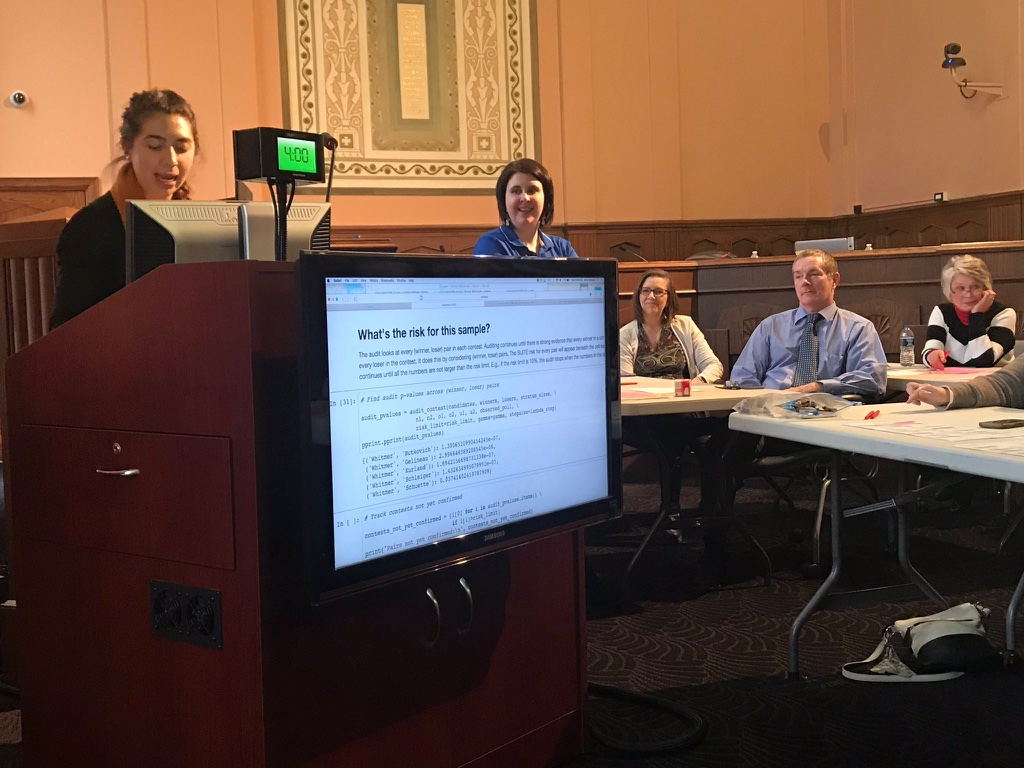
\includegraphics[width=0.9\linewidth]{../photo/notebook}
\end{figure}

%------------------------------------------------




%----------------------------------------------------------------------------------------

\end{column} % End of the first column

\begin{column}{\sepwid}\end{column} % Empty spacer column

\begin{column}{\twocolwid} % Begin a column which is two columns wide (column 2)

\begin{columns}[t,totalwidth=\twocolwid] % Split up the two columns wide column

\begin{column}{\onecolwid}\vspace{-.6in} % The first column within column 2 (column 2.1)

%----------------------------------------------------------------------------------------
%	DATA
%----------------------------------------------------------------------------------------

\begin{block}{The SUITE Tool}

I created a Jupyter notebook to run calculations for a two-stratum SUITE audit from start to finish.

\begin{itemize}
\item Estimate initial sample sizes in each stratum based on reported results
\item Sample ballots using a cryptographically-secure pseudo-random number generator
\item Run the risk calculations for the observed samples
\item Log each step in a JSON file 
\end{itemize}
\end{block}

\begin{alertblock}{Use the Tool}
Find a link to run the SUITE tool interactively at \href{https://www.github.com/pbstark/CORLA18}{https://www.github.com/pbstark/CORLA18}. 
\end{alertblock}


%----------------------------------------------------------------------------------------

\end{column} % End of column 2.1

\begin{column}{\onecolwid}\vspace{-.6in} % The second column within column 2 (column 2.2)

%----------------------------------------------------------------------------------------
%	METHODS
%----------------------------------------------------------------------------------------

\begin{block}{Michigan Pilots}
\begin{itemize}
\item 8 RLA experts traveled to 3 cities with the Bureau of Elections to pilot RLAs after the Nov. 2018 elections \\
\item Used SUITE to combine ballot polling for election day ballots with ballot-level comparison
for absentee ballots
\end{itemize}

\begin{table}[h]
\begin{center}
\begin{tabular}{l|rrrrrrr}
City & Total  & Margin &   Absentee    & \# Ballots  \\
       & ballots &             &   rate                    & audited  \\
\hline
Rochester Hills & 36,666 & 29\% & 0\% & 76 \\
Lansing & 21,328 & 12\% & 50\% & 260 \\
Kalamazoo & 27,666 & 55\% & 19\% & 40 
\end{tabular}
%\caption{Summary of the races audited. Ballots and votes for the candidates are the results as reported.
%Margins are expressed as a percentage of total ballots cast.
%The ballots included in the contest under audit in Lansing were restricted for the purpose of the pilot;
%half of Election Day precincts were omitted.}
\end{center}
\label{tab:audit_summary}
\end{table}%

\end{block}

%----------------------------------------------------------------------------------------

\end{column} % End of column 2.2

\end{columns} % End of the split of column 2 - any content after this will now take up 2 columns width

%----------------------------------------------------------------------------------------
%	IMPORTANT RESULT
%----------------------------------------------------------------------------------------

%\begin{alertblock}{Challenges}
%\begin{center}
%Communication between academic researchers and election officials is critical to resolving barriers to implementing RLAs.
%\end{center}
%\end{alertblock} 

%----------------------------------------------------------------------------------------

\begin{columns}[t,totalwidth=\twocolwid] % Split up the two columns wide column again

\begin{column}{\onecolwid} % The first column within column 2 (column 2.1)

%----------------------------------------------------------------------------------------
% 	RESULTS column 1
%----------------------------------------------------------------------------------------

\begin{block}{Creating the Ballot Manifest}

\begin{itemize}
\item Stratified sampling requires a sampling frame for each stratum
\item Record number of ballots in each physical grouping (``batch'')
\end{itemize}
\begin{figure}
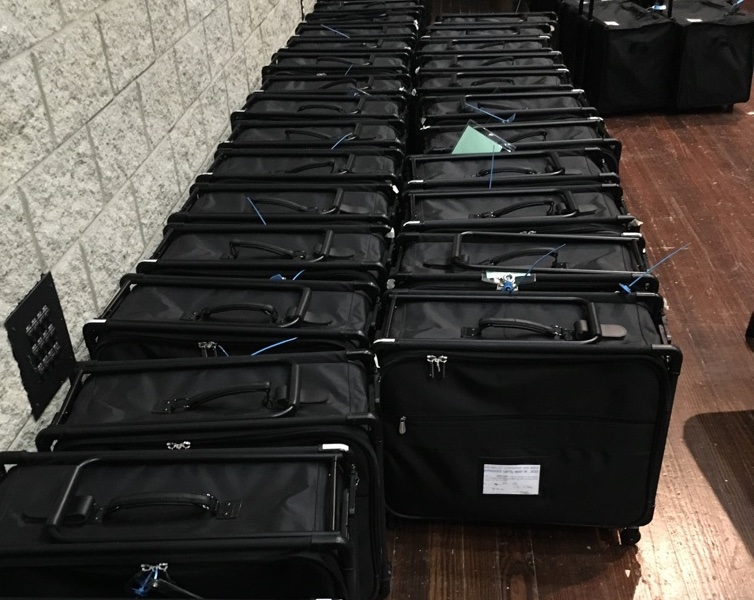
\includegraphics[width=0.7\linewidth]{../photo/ballotbags}
\end{figure}
\end{block}

\begin{block}{Cast Vote Record Files}
\begin{itemize}
\item Records to link absentee votes on paper to their electronic interpretation
\item Files are voting system dependent and difficult to process (e.g. JSON files with unintuitive coding)
\item Election officials need to work with vendors to obtain human-readable files
\end{itemize}
\end{block}

%----------------------------------------------------------------------------------------

\end{column} % End of column 2.1

\begin{column}{\onecolwid} % The second column within column 2 (column 2.2)

%----------------------------------------------------------------------------------------
%	RESULTS column 2
%----------------------------------------------------------------------------------------

\begin{block}{Retrieving Ballots}

\begin{itemize}
\item Locating the sampled ballot in a large batch is inefficient
\item $k$-cut: shuffle batch like a deck of cards to approximate sampling \cite{sridhar_kcut_2018}
\end{itemize}
\begin{figure}
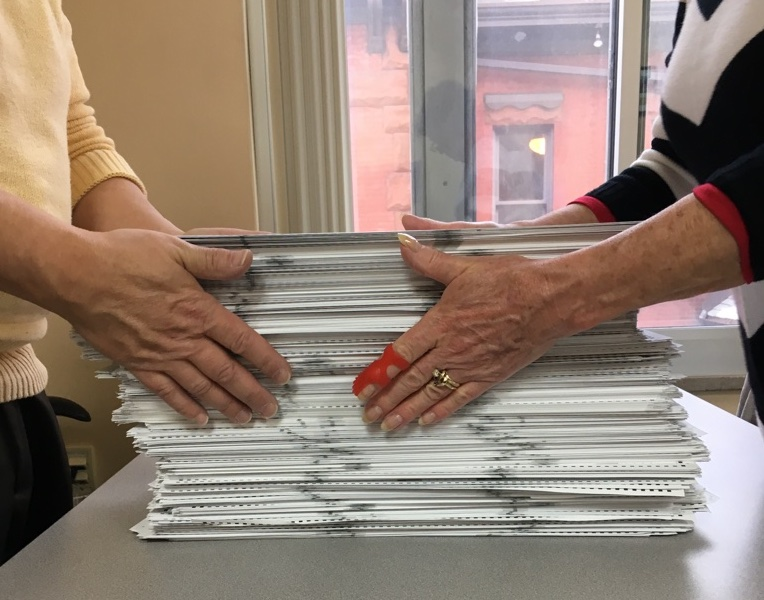
\includegraphics[width=0.7\linewidth]{../photo/batch}
\end{figure}
\end{block}


\begin{block}{Paper Handling}
\begin{itemize}
\item Matching paper ballots to their cast vote records can be challenging
\item Method 1: Store ballots in same order in which they were scanned (difficult)
\item Method 2: imprint with a unique ID (security and anonymity concerns)
\end{itemize}
\end{block}

%----------------------------------------------------------------------------------------

\end{column} % End of column 2.2

\end{columns} % End of the split of column 2

%
%\begin{center}
%\small\rmfamily
%\begin{tabular}{| l | c  c | c  c |}
%\toprule
%& \textbf{Alcohol} & & \textbf{Salt} & \\ \hline
% & {Correlation} & {P-value}& {Correlation} & {P-value}\\
%\midrule
%Males & 0.4997 & 0.0014 & 0.003 & 0.4835 \\
%Females & 0.4294 & 0.0051 & -0.2640 & 0.9382 \\
%\bottomrule
%\end{tabular}
%\end{center}

\end{column} % End of the second column

\begin{column}{\sepwid}\end{column} % Empty spacer column

\begin{column}{\onecolwid} % The third column

%----------------------------------------------------------------------------------------
%	CONCLUSION
%----------------------------------------------------------------------------------------

\begin{block}{Conclusions}

Pilot audits are critical to making RLAs the norm.

\begin{itemize}
\item Give election officials confidence in the process
\item Shed light on practical barriers and unanticipated problems
\item Demonstrate their efficiency over existing approaches
\end{itemize}
\end{block}

%----------------------------------------------------------------------------------------
%	REFERENCES
%----------------------------------------------------------------------------------------

\begin{block}{References}

\nocite{*} % Insert publications even if they are not cited in the poster
\small{\bibliographystyle{unsrt}
\bibliography{refs}\vspace{0.75in}}

\end{block}
%
%%----------------------------------------------------------------------------------------
%%	ACKNOWLEDGEMENTS
%%----------------------------------------------------------------------------------------
%
%\setbeamercolor{block title}{fg=red,bg=white} % Change the block title color

\begin{block}{Acknowledgements}

I'd like to thank many people who made this project a success:
\begin{itemize}
\item Philip Stark, Mark Lindeman, Neal McBurnett, and the ElectionAuditWare group for helpful suggestions on the math and SUITE tool
\item The city clerks and state election officials in Michigan for inviting me to their pilots and their willingness to try the unknown
\item Berkeley Institute for Data Science for supporting my travel to Michigan
\item EVN for their recognition of the SUITE tool with their annual Innovation Award
\end{itemize}

\end{block}

%----------------------------------------------------------------------------------------
%	CONTACT INFORMATION
%----------------------------------------------------------------------------------------

%\setbeamercolor{block alerted title}{fg=black,bg=norange} % Change the alert block title colors
%\setbeamercolor{block alerted body}{fg=black,bg=white} % Change the alert block body colors

\begin{alertblock}{Contact Information}
Email: \href{mailto:kellieotto@berkeley.edu}{kellieotto@berkeley.edu} \\
Website: \href{www.kellieottoboni.com}{www.kellieottoboni.com}\\
Twitter: @kellieotto
\end{alertblock}



%----------------------------------------------------------------------------------------

\end{column} % End of the third column

\end{columns} % End of all the columns in the poster

\end{frame} % End of the enclosing frame

\end{document}
